% Source reference: :contentReference[oaicite:0]{index=0}
\part{Graph Theory}
\section{Handout 07: Graph Theory (1)}

\subsection{Overview}

This handout begins Part~III of the course. The emphasis is foundational: we introduce the language of graphs, basic graph invariants, and the notion of graph isomorphism. The main topics are:
\begin{itemize}[leftmargin=*]
    \item graph models and formal graph definitions;
    \item vertices, edges, adjacency, incidence, and degree;
    \item simple graphs, multigraphs, complete graphs, and cycle graphs;
    \item subgraphs and induced subgraphs;
    \item graph isomorphism and graph invariants;
    \item the Handshaking Lemma and its first consequences.
\end{itemize}

The guiding principle is that a graph is an abstract structure encoding \emph{objects} together with \emph{relationships} between them.

\begin{examtip}[title={Main mindset for Handout 07}]
A graph drawing is only a picture of an abstract object. The location of the vertices on the page, the length of edges, and whether edges are curved or straight are usually irrelevant. What matters is which vertices are connected to which.
\end{examtip}

%==================================================
\subsection{Graph Models}
%==================================================

Many real-world systems naturally lead to graphs:
\begin{itemize}[leftmargin=*]
    \item in an MRT map, stations are vertices and track connections are edges;
    \item in a friendship network, people are vertices and friendships are edges;
    \item in a molecule, atoms are vertices and chemical bonds are edges;
    \item in a flowchart, states or actions are vertices and transitions are directed edges;
    \item in the Bridges of Königsberg problem, land masses may be treated as vertices and bridges as edges.
\end{itemize}

\begin{examplebox}[title={Why these examples belong to one framework}]
In each case there is:
\begin{enumerate}[leftmargin=*]
    \item a collection of objects; and
    \item a specification of which pairs of objects are related.
\end{enumerate}
This is precisely what a graph records.
\end{examplebox}

\begin{extension}[title={Abstraction step in graph theory}]
Graph theory becomes powerful only after irrelevant geometric information is discarded. For example, an MRT map and a completely redrawn version of the same network represent the same graph if the adjacency structure is unchanged.
\end{extension}

%==================================================
\subsection{Undirected and Directed Graphs}
%==================================================

\begin{definition}{Undirected graph}{undirected-graph}
An \emph{undirected graph} is an ordered pair
\[
G=(V,E),
\]
where:
\begin{itemize}[leftmargin=*]
    \item \(V\) is a nonempty set of vertices; and
    \item \(E\) is a set of edges, where each edge has one or two endpoints in \(V\).
\end{itemize}
In a simple undirected graph, each edge is an unordered pair \(\{u,v\}\) of distinct vertices.
\end{definition}

\begin{definition}{Directed graph}{directed-graph}
A \emph{directed graph} (or \emph{digraph}) is an ordered pair
\[
G=(V,E),
\]
where \(V\) is a nonempty set of vertices and each edge in \(E\) is an ordered pair \((u,v)\), called a directed edge from \(u\) to \(v\).
\end{definition}

% Comparison of undirected and directed edges between labelled vertices.
\begin{center}
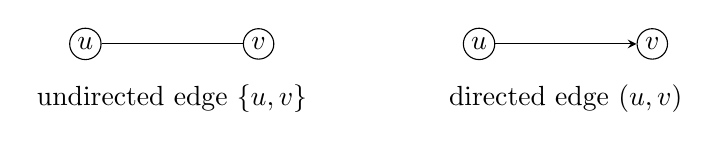
\begin{tikzpicture}[>=stealth,scale=1]
    \node[circle,draw,inner sep=1.5pt] (u1) at (0,0) {$u$};
    \node[circle,draw,inner sep=1.5pt] (v1) at (2.2,0) {$v$};
    \draw[-] (u1) -- (v1);
    \node at (1.1,-0.7) {undirected edge $\{u,v\}$};

    \node[circle,draw,inner sep=1.5pt] (u2) at (5,0) {$u$};
    \node[circle,draw,inner sep=1.5pt] (v2) at (7.2,0) {$v$};
    \draw[->] (u2) -- (v2);
    \node at (6.1,-0.7) {directed edge $(u,v)$};
\end{tikzpicture}
\end{center}

\begin{commonmistake}[title={Ordered pair versus unordered pair}]
In an undirected graph,
\[
\{u,v\}=\{v,u\},
\]
but in a digraph,
\[
(u,v)\neq (v,u)
\]
in general. The notation determines the meaning.
\end{commonmistake}

%==================================================
\subsection{Simple Graphs and Multigraphs}
%==================================================

\begin{definition}{Simple graph}{simple-graph}
An undirected graph is called \emph{simple} if:
\begin{itemize}[leftmargin=*]
    \item no self-loop \(\{v,v\}\) is allowed;
    \item there is at most one edge between any two distinct vertices.
\end{itemize}
\end{definition}

\begin{definition}{Multigraph}{multigraph}
A \emph{multigraph} is a graph in which self-loops and/or multiple edges between the same pair of vertices are allowed.
\end{definition}

If \(G=(V,E)\) is a simple graph and
\[
n=|V|,\qquad m=|E|,
\]
then every edge is determined by a choice of two distinct vertices, so
\[
0\le m\le \binom{n}{2}.
\]

\begin{keyformula}[title={Edge bound for a simple graph}]
If \(G\) is a simple graph with \(n\) vertices, then
\[
0\le |E|\le \binom{n}{2}.
\]
The upper bound is attained exactly by the complete graph \(K_n\).
\end{keyformula}

\begin{examtip}[title={Default convention in MH1301}]
Unless stated otherwise, graphs in the lectures, tutorials, and exams are assumed to be \emph{simple} graphs.
\end{examtip}

%==================================================
\subsection{Adjacency, Incidence, and Endpoints}
%==================================================

\begin{definition}{Adjacency and incidence}{adjacency-incidence}
Let \(G=(V,E)\) be an undirected graph.
\begin{itemize}[leftmargin=*]
    \item Two vertices \(u,v\in V\) are \emph{adjacent} (or \emph{neighbors}) if \(\{u,v\}\in E\).
    \item If \(e=\{u,v\}\in E\), then \(e\) is \emph{incident} with \(u\) and \(v\).
    \item The vertices \(u\) and \(v\) are called the \emph{endpoints} of \(e\).
\end{itemize}
\end{definition}

% Small labelled graph for adjacency and incidence examples.
\begin{center}
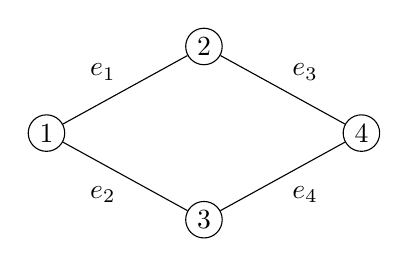
\begin{tikzpicture}[scale=1,>=stealth]
    \node[circle,draw,inner sep=1.8pt] (1) at (0,0) {$1$};
    \node[circle,draw,inner sep=1.8pt] (2) at (2,1.1) {$2$};
    \node[circle,draw,inner sep=1.8pt] (3) at (2,-1.1) {$3$};
    \node[circle,draw,inner sep=1.8pt] (4) at (4,0) {$4$};
    \draw (1) -- node[above left] {$e_1$} (2);
    \draw (1) -- node[below left] {$e_2$} (3);
    \draw (2) -- node[above right] {$e_3$} (4);
    \draw (3) -- node[below right] {$e_4$} (4);
\end{tikzpicture}
\end{center}

\begin{examplebox}[title={Reading adjacency and incidence from a graph}]
In the graph above:
\begin{itemize}[leftmargin=*]
    \item vertices \(1\) and \(2\) are adjacent;
    \item the edge \(e_1\) is incident with vertices \(1\) and \(2\);
    \item vertex \(1\) is an endpoint of \(e_1\) and \(e_2\).
\end{itemize}
Adjacency is a relation between vertices; incidence is a relation between a vertex and an edge.
\end{examplebox}

%==================================================
\subsection{Degree of a Vertex}
%==================================================

\begin{definition}{Degree}{degree-def}
Let \(G=(V,E)\) be a graph.
\begin{itemize}[leftmargin=*]
    \item The \emph{degree} of a vertex \(v\in V\), denoted \(\deg(v)\), is the number of edges incident with \(v\).
    \item The \emph{degree of the graph}, denoted \(\deg(G)\), is the maximum degree of its vertices.
    \item A vertex of degree \(0\) is called \emph{isolated}.
    \item If every vertex has degree \(k\), then the graph is called \emph{\(k\)-regular}.
\end{itemize}
If a self-loop occurs in a multigraph, it contributes \(2\) to the degree of its vertex.
\end{definition}

\begin{examplebox}[title={Degrees in the displayed graph}]
For the graph in the previous figure,
\[
\deg(1)=2,\qquad \deg(2)=2,\qquad \deg(3)=2,\qquad \deg(4)=2.
\]
Hence the graph is \(2\)-regular.
\end{examplebox}

\begin{examplebox}[title={An isolated vertex}]
If a graph contains a vertex with no incident edges at all, then that vertex has degree \(0\) and is isolated.
\end{examplebox}

\begin{commonmistake}[title={A loop contributes two, not one}]
In a multigraph, a self-loop begins and ends at the same vertex, so it contributes \(2\) to the degree count of that vertex.
\end{commonmistake}

%==================================================
\subsection{The Handshaking Lemma}
%==================================================

\begin{theorem}{Handshaking Lemma}{handshaking}
Let \(G=(V,E)\) be an undirected graph with \(m\) edges. Then
\[
\sum_{v\in V}\deg(v)=2m.
\]
\end{theorem}

\begin{proof}
Each edge has two endpoints, so each edge contributes exactly \(2\) to the total degree count of all vertices. Summing over all edges, the total contribution is \(2m\). Therefore
\[
\sum_{v\in V}\deg(v)=2m.
\]
\end{proof}

\begin{keyformula}[title={Handshaking Lemma}]
\[
2|E|=\sum_{v\in V}\deg(v).
\]
\end{keyformula}

\begin{examplebox}[title={Example 3 from the handout}]
How many edges are there in a \(6\)-regular graph with \(10\) vertices?

Let \(m\) be the number of edges. Since every vertex has degree \(6\),
\[
\sum_{v\in V}\deg(v)=10\cdot 6=60.
\]
By the Handshaking Lemma,
\[
2m=60,
\]
so
\[
\boxed{m=30.}
\]
\end{examplebox}

\begin{theorem}{Odd-degree vertices occur in even number}{odd-degree-even-count}
In every undirected graph, the number of vertices of odd degree is even.
\end{theorem}

\begin{proof}
By the Handshaking Lemma,
\[
\sum_{v\in V}\deg(v)=2|E|,
\]
which is even. The sum of all even-degree vertices is even. Therefore the sum of the odd degrees must also be even. A sum of odd integers is even if and only if there are an even number of them. Hence the number of odd-degree vertices is even.
\end{proof}

\begin{examplebox}[title={Tutorial 7, Question 4}]
Show that in a simple graph with at least two vertices, two vertices must have the same degree.

Let the graph have \(n\ge 2\) vertices. Each degree lies in the set
\[
\{0,1,2,\dots,n-1\}.
\]
However, a simple graph cannot simultaneously contain:
\begin{itemize}[leftmargin=*]
    \item a vertex of degree \(0\), and
    \item a vertex of degree \(n-1\).
\end{itemize}
Indeed, a degree-\((n-1)\) vertex is adjacent to every other vertex, so no vertex can be isolated.

Hence the \(n\) vertices can realize at most \(n-1\) distinct degree values. By the pigeonhole principle, two vertices must have the same degree.
\end{examplebox}

\begin{extension}[title={Why the Handshaking Lemma is powerful}]
The lemma turns a local quantity, degree, into a global counting identity. Many impossibility results in graph theory are obtained by showing that the degree data violate parity or edge-count constraints coming from
\[
\sum_{v\in V}\deg(v)=2|E|.
\]
\end{extension}

%==================================================
\subsection{Special Graphs}
%==================================================

\subsubsection{Complete graphs}

\begin{definition}{Complete graph}{complete-graph}
The \emph{complete graph} on \(n\) vertices, denoted \(K_n\), is the simple graph in which every pair of distinct vertices is connected by an edge.
\end{definition}

Every vertex of \(K_n\) is adjacent to all other \(n-1\) vertices. Hence \(K_n\) is \((n-1)\)-regular and
\[
|E(K_n)|=\binom{n}{2}.
\]

% First few complete graphs K1 to K4.
\begin{center}
\begin{tikzpicture}[scale=0.9]
    \node[circle,draw,inner sep=1.4pt] at (0,0) {};
    \node at (0,-1) {$K_1$};

    \begin{scope}[shift={(2.7,0)}]
        \node[circle,draw,inner sep=1.4pt] (a) at (0,0) {};
        \node[circle,draw,inner sep=1.4pt] (b) at (1.2,0) {};
        \draw (a)--(b);
        \node at (0.6,-1) {$K_2$};
    \end{scope}

    \begin{scope}[shift={(6.2,0)}]
        \node[circle,draw,inner sep=1.4pt] (a) at (0,0.75) {};
        \node[circle,draw,inner sep=1.4pt] (b) at (-0.7,-0.45) {};
        \node[circle,draw,inner sep=1.4pt] (c) at (0.7,-0.45) {};
        \draw (a)--(b)--(c)--(a);
        \node at (0,-1.2) {$K_3$};
    \end{scope}

    \begin{scope}[shift={(10.6,0)}]
        \node[circle,draw,inner sep=1.4pt] (a) at (-0.7,0.7) {};
        \node[circle,draw,inner sep=1.4pt] (b) at (0.7,0.7) {};
        \node[circle,draw,inner sep=1.4pt] (c) at (-0.7,-0.7) {};
        \node[circle,draw,inner sep=1.4pt] (d) at (0.7,-0.7) {};
        \draw (a)--(b)--(d)--(c)--(a)--(d) (b)--(c);
        \node at (0,-1.4) {$K_4$};
    \end{scope}
\end{tikzpicture}
\end{center}

\subsubsection{Cycle graphs}

\begin{definition}{Cycle graph}{cycle-graph}
For \(n\ge 3\), the \emph{cycle graph} \(C_n\) has vertices \(v_1,\dots,v_n\) and edge set
\[
\{\{v_1,v_2\},\{v_2,v_3\},\dots,\{v_{n-1},v_n\},\{v_n,v_1\}\}.
\]
\end{definition}

Every cycle graph is \(2\)-regular.

% First few cycle graphs C3 to C5.
\begin{center}
\begin{tikzpicture}[scale=0.9]
    \begin{scope}[shift={(0,0)}]
        \node[circle,draw,inner sep=1.4pt] (a) at (0,0.9) {};
        \node[circle,draw,inner sep=1.4pt] (b) at (-0.8,-0.45) {};
        \node[circle,draw,inner sep=1.4pt] (c) at (0.8,-0.45) {};
        \draw (a)--(b)--(c)--(a);
        \node at (0,-1.25) {$C_3$};
    \end{scope}
    \begin{scope}[shift={(4,0)}]
        \node[circle,draw,inner sep=1.4pt] (a) at (-0.8,0.8) {};
        \node[circle,draw,inner sep=1.4pt] (b) at (0.8,0.8) {};
        \node[circle,draw,inner sep=1.4pt] (c) at (0.8,-0.8) {};
        \node[circle,draw,inner sep=1.4pt] (d) at (-0.8,-0.8) {};
        \draw (a)--(b)--(c)--(d)--(a);
        \node at (0,-1.35) {$C_4$};
    \end{scope}
    \begin{scope}[shift={(8.5,0)}]
        \foreach \i/\x/\y in {1/0/1,2/0.95/0.3,3/0.58/-0.82,4/-0.58/-0.82,5/-0.95/0.3}
            \node[circle,draw,inner sep=1.4pt] (v\i) at (\x,\y) {};
        \draw (v1)--(v2)--(v3)--(v4)--(v5)--(v1);
        \node at (0,-1.35) {$C_5$};
    \end{scope}
\end{tikzpicture}
\end{center}

\begin{examplebox}[title={Degrees in special graphs}]
For \(K_n\), every vertex has degree \(n-1\).
For \(C_n\), every vertex has degree \(2\).
Hence
\[
\deg(K_n)=n-1,
\qquad
\deg(C_n)=2.
\]
\end{examplebox}

%==================================================
\subsection{Subgraphs and Induced Subgraphs}
%==================================================

\begin{definition}{Subgraph}{subgraph-def}
A graph \(H=(W,F)\) is a \emph{subgraph} of a graph \(G=(V,E)\) if
\[
W\subseteq V
\qquad\text{and}\qquad
F\subseteq E.
\]
\end{definition}

\begin{definition}{Induced subgraph}{induced-subgraph}
A subgraph \(H=(W,F)\) of \(G=(V,E)\) is an \emph{induced subgraph} if \(F\) contains \emph{all} edges of \(G\) whose endpoints both lie in \(W\).
\end{definition}

% Subgraph versus induced subgraph on the same vertex subset.
\begin{center}
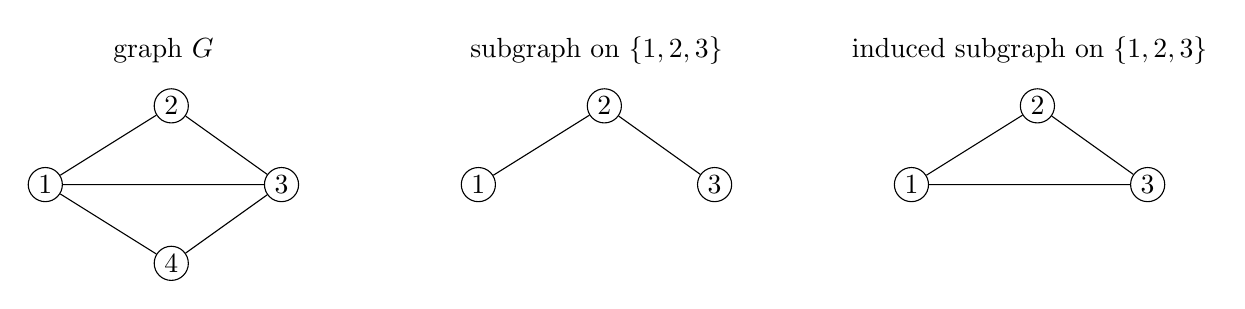
\begin{tikzpicture}[scale=1]
    \begin{scope}[shift={(0,0)}]
        \node at (1.5,1.7) {graph $G$};
        \node[circle,draw,inner sep=1.5pt] (1) at (0,0) {$1$};
        \node[circle,draw,inner sep=1.5pt] (2) at (1.6,1.0) {$2$};
        \node[circle,draw,inner sep=1.5pt] (3) at (3.0,0) {$3$};
        \node[circle,draw,inner sep=1.5pt] (4) at (1.6,-1.0) {$4$};
        \draw (1)--(2)--(3)--(4)--(1)--(3);
    \end{scope}
    \begin{scope}[shift={(5.5,0)}]
        \node at (1.5,1.7) {subgraph on $\{1,2,3\}$};
        \node[circle,draw,inner sep=1.5pt] (1) at (0,0) {$1$};
        \node[circle,draw,inner sep=1.5pt] (2) at (1.6,1.0) {$2$};
        \node[circle,draw,inner sep=1.5pt] (3) at (3.0,0) {$3$};
        \draw (1)--(2)--(3);
    \end{scope}
    \begin{scope}[shift={(11,0)}]
        \node at (1.5,1.7) {induced subgraph on $\{1,2,3\}$};
        \node[circle,draw,inner sep=1.5pt] (1) at (0,0) {$1$};
        \node[circle,draw,inner sep=1.5pt] (2) at (1.6,1.0) {$2$};
        \node[circle,draw,inner sep=1.5pt] (3) at (3.0,0) {$3$};
        \draw (1)--(2)--(3)--(1);
    \end{scope}
\end{tikzpicture}
\end{center}

\begin{examplebox}[title={Subgraph versus induced subgraph}]
Choose vertices \(\{1,2,3\}\) from the graph displayed above. If one keeps only some of the edges among these three vertices, one gets a subgraph. If one keeps \emph{all} edges of the original graph between these chosen vertices, one gets the induced subgraph.
\end{examplebox}

\begin{commonmistake}[title={Not every subgraph is induced}]
An induced subgraph is determined entirely by its vertex subset. A general subgraph is not: after choosing vertices, one may still omit edges that were present in the original graph.
\end{commonmistake}

%==================================================
\subsection{Graph Isomorphism}
%==================================================

\begin{definition}{Graph isomorphism}{graph-isomorphism}
Two undirected graphs
\[
G_1=(V_1,E_1)
\qquad\text{and}\qquad
G_2=(V_2,E_2)
\]
are \emph{isomorphic} if there exists a bijection
\[
f:V_1\to V_2
\]
such that for all \(u,v\in V_1\),
\[
\{u,v\}\in E_1
\iff
\{f(u),f(v)\}\in E_2.
\]
\end{definition}

Intuitively, isomorphic graphs are the same graph with different vertex labels.

\begin{examplebox}[title={A concrete isomorphism}]
Let
\[
V_1=\{a,b,c,d\},
\qquad
V_2=\{r,s,t,u\},
\]
and suppose the edges in the two graphs correspond as follows:
\[
f(a)=r,\qquad f(b)=s,\qquad f(c)=u,\qquad f(d)=t.
\]
If adjacency is preserved under this bijection, then the graphs are isomorphic.
\end{examplebox}

\begin{examtip}[title={How to prove two graphs are isomorphic}]
To prove two graphs are isomorphic, one must produce an explicit bijection between their vertex sets and check that adjacency is preserved in both directions.
\end{examtip}

\subsubsection{Graph invariants}

A \emph{graph invariant} is a property preserved by isomorphism. Common invariants include:
\begin{itemize}[leftmargin=*]
    \item number of vertices;
    \item number of edges;
    \item number of isolated vertices;
    \item degree sequence;
    \item regularity.
\end{itemize}

\begin{examplebox}[title={Showing graphs are not isomorphic}]
If one graph has degree sequence
\[
(3,2,2,1)
\]
and another has degree sequence
\[
(3,3,1,1),
\]
then the graphs cannot be isomorphic, because degree sequence is an invariant.
\end{examplebox}

\begin{examplebox}[title={Handout non-isomorphism example}]
The handout gives a pair of graphs \(G\) and \(H\) and notes that a vertex of degree \(2\) in \(G\) is adjacent to two vertices of degree \(3\), while no degree-\(2\) vertex in \(H\) has that property. Hence the graphs are not isomorphic.

This illustrates a common strategy: compare \emph{local adjacency patterns} among vertices of the same degree.
\end{examplebox}

\begin{extension}[title={Why isomorphism can be difficult}]
For two graphs with \(n\) vertices there are \(n!\) possible bijections between the vertex sets. Brute-force checking is therefore impractical even for moderate \(n\). In practice one first uses invariants to rule out isomorphism quickly, and only then searches for an explicit bijection if the invariants are compatible.
\end{extension}

%==================================================
\subsection{Special Techniques}
%==================================================

\subsubsection*{1. Ignore the picture, read the adjacency}
Different drawings can represent the same graph. Always extract the vertex set and edge set, not the visual layout.

\subsubsection*{2. Use the Handshaking Lemma early}
Whenever degrees and edge counts appear together, immediately consider
\[
\sum_{v\in V}\deg(v)=2|E|.
\]
This often gives the shortest solution.

\subsubsection*{3. Use invariants to disprove isomorphism}
To show two graphs are not isomorphic, compare quick invariants such as:
\begin{itemize}[leftmargin=*]
    \item number of vertices;
    \item number of edges;
    \item degree sequence;
    \item number of isolated vertices;
    \item adjacency pattern among high-degree vertices.
\end{itemize}

\subsubsection*{4. For isomorphism, build a bijection strategically}
Match vertices of uncommon degree first. Then check whether their neighborhoods correspond.

\subsubsection*{5. Distinguish subgraph from induced subgraph}
A subgraph may omit edges. An induced subgraph may not omit any edge whose endpoints remain in the chosen vertex set.

\subsubsection*{6. Check parity of odd degrees}
If a proposed degree pattern contains an odd number of odd entries, then it cannot come from any graph.

\begin{examtip}[title={Fast diagnostic summary}]
When facing a graph question, ask in this order:
\begin{enumerate}[leftmargin=*]
    \item Is the graph simple or directed?
    \item What are \(|V|\) and \(|E|\)?
    \item What are the degrees of the vertices?
    \item Can the Handshaking Lemma be applied?
    \item Is the task about equality of drawings, or about isomorphism of abstract graphs?
\end{enumerate}
\end{examtip}

%==================================================
\subsection{Summary Table}
%==================================================

\begin{center}
\small
\begin{tabular}{@{}p{0.27\textwidth}p{0.28\textwidth}p{0.34\textwidth}@{}}
\toprule
\textbf{Concept} & \textbf{Formal object} & \textbf{Key point} \\
\midrule
Undirected graph & \(G=(V,E)\) with edges as unordered pairs & adjacency is symmetric \\
Directed graph & \(G=(V,E)\) with edges as ordered pairs & direction matters \\
Simple graph & no loops, no multiple edges & \(0\le |E|\le \binom{|V|}{2}\) \\
Degree & \(\deg(v)\) & number of incident edges \\
Regular graph & all vertices same degree & \(k\)-regular means \(\deg(v)=k\) for all \(v\) \\
Handshaking Lemma & \(2|E|=\sum_{v\in V}\deg(v)\) & total degree count is even \\
Complete graph & \(K_n\) & every pair of vertices adjacent \\
Cycle graph & \(C_n\) & every vertex has degree \(2\) \\
Subgraph & \(W\subseteq V,\ F\subseteq E\) & may omit edges \\
Induced subgraph & determined by chosen vertex subset & keeps all edges among chosen vertices \\
Isomorphism & adjacency-preserving bijection & same abstract graph, different labels \\
\bottomrule
\end{tabular}
\end{center}

\begin{commonmistake}[title={Final warning for Handout 07}]
A graph question is rarely about the artistic appearance of a drawing. It is about the combinatorial structure: which vertices are present, which edges are present, and how these determine adjacency, degree, and isomorphism.
\end{commonmistake}